\documentclass[12pt]{report}
\usepackage[margin=1in]{geometry}
\usepackage{setspace} % for single/doublespacing commands
\usepackage{graphicx} % including graphics
\usepackage{sectsty} % sexy section headings
\usepackage{pdfpages} % including multipage pdfs
\usepackage[export]{adjustbox} % for graphic frames and center
\usepackage{siunitx}
\usepackage[numbered]{matlab-prettifier} % including matlab w/ syntax highlighting
\usepackage[T1]{fontenc} % prettier matlab font
\usepackage{xfrac} % more legible inline fractions (\sfrac)
\usepackage{lmodern} % font package for above
\usepackage{multicol} % multiple columns
\usepackage[justification=centering]{caption} % figure captions (force centering)
\usepackage{amsmath} % more math symbols and shit
\usepackage{enumitem} % add arguments for enumerate to change style
\usepackage[list=true]{subcaption} % subfigures with list of figure support
\usepackage{multirow}
\usepackage{mathtools}
\usepackage{booktabs}
\usepackage{color}
\usepackage{ulem}
\usepackage{blindtext}
\usepackage{natbib}
\usepackage{contour}
\usepackage{tabularx}
\usepackage{circuitikz} % drawing fancy shit
\usepackage{cancel} % arrow and cross math cancel symbol
\usepackage{lineno}
\usepackage{framed}
\usepackage{amssymb} % special math symbols
\usepackage{listings}
\usepackage{array}
\usepackage{BOONDOX-cal} % fancy mathtype script
\usepackage{fancyhdr}

\renewcommand{\bibname}{References}
\sisetup{output-exponent-marker=\ensuremath{\mathrm{e}}}
\newcommand{\PreserveBackslash}[1]{\let\temp=\\#1\let\\=\temp}
\newcolumntype{C}[1]{>{\PreserveBackslash\centering}p{#1}}
\newcolumntype{R}[1]{>{\PreserveBackslash\raggedleft}p{#1}}
\newcolumntype{L}[1]{>{\PreserveBackslash\raggedright}p{#1}}
\lstMakeShortInline[style=Matlab-editor]| % matlab inline escape character
\graphicspath{{images/}}
\renewcommand\thesection{\arabic{section}}
\renewcommand\labelitemi{---}
\lstset{numberstyle=\ttfamily\small\color{gray}}
\renewcommand\linenumberfont{\ttfamily\small\color{gray}}
\setlength\linenumbersep{6mm}
% \hbadness=99999  % or any number >=10000
\usetikzlibrary{arrows,calc,patterns,angles,quotes}
\usetikzlibrary{decorations.pathmorphing,decorations.pathreplacing} % for snakes!
\newcommand{\Lag}{\mathcal{L}} % lagrangian L
% \titlespacing{command}{left spacing}{before spacing}{after spacing}[right]

% \titlespacing\subsection{0pt}{12pt plus 4pt minus 2pt}{0pt plus 2pt minus 2pt}
% \titlespacing\subsubsection{0pt}{12pt plus 4pt minus 2pt}{0pt plus 2pt minus 2pt}

\begin{document}
\normalem
\begin{titlepage}
\flushleft
\doublespacing
\Large
\textsc{Test Document} \\
\normalsize
Trey Dufrene, Zack Johnson, David Orcutt, Alan Wallingford, Ryan Warner
\vfill
\center
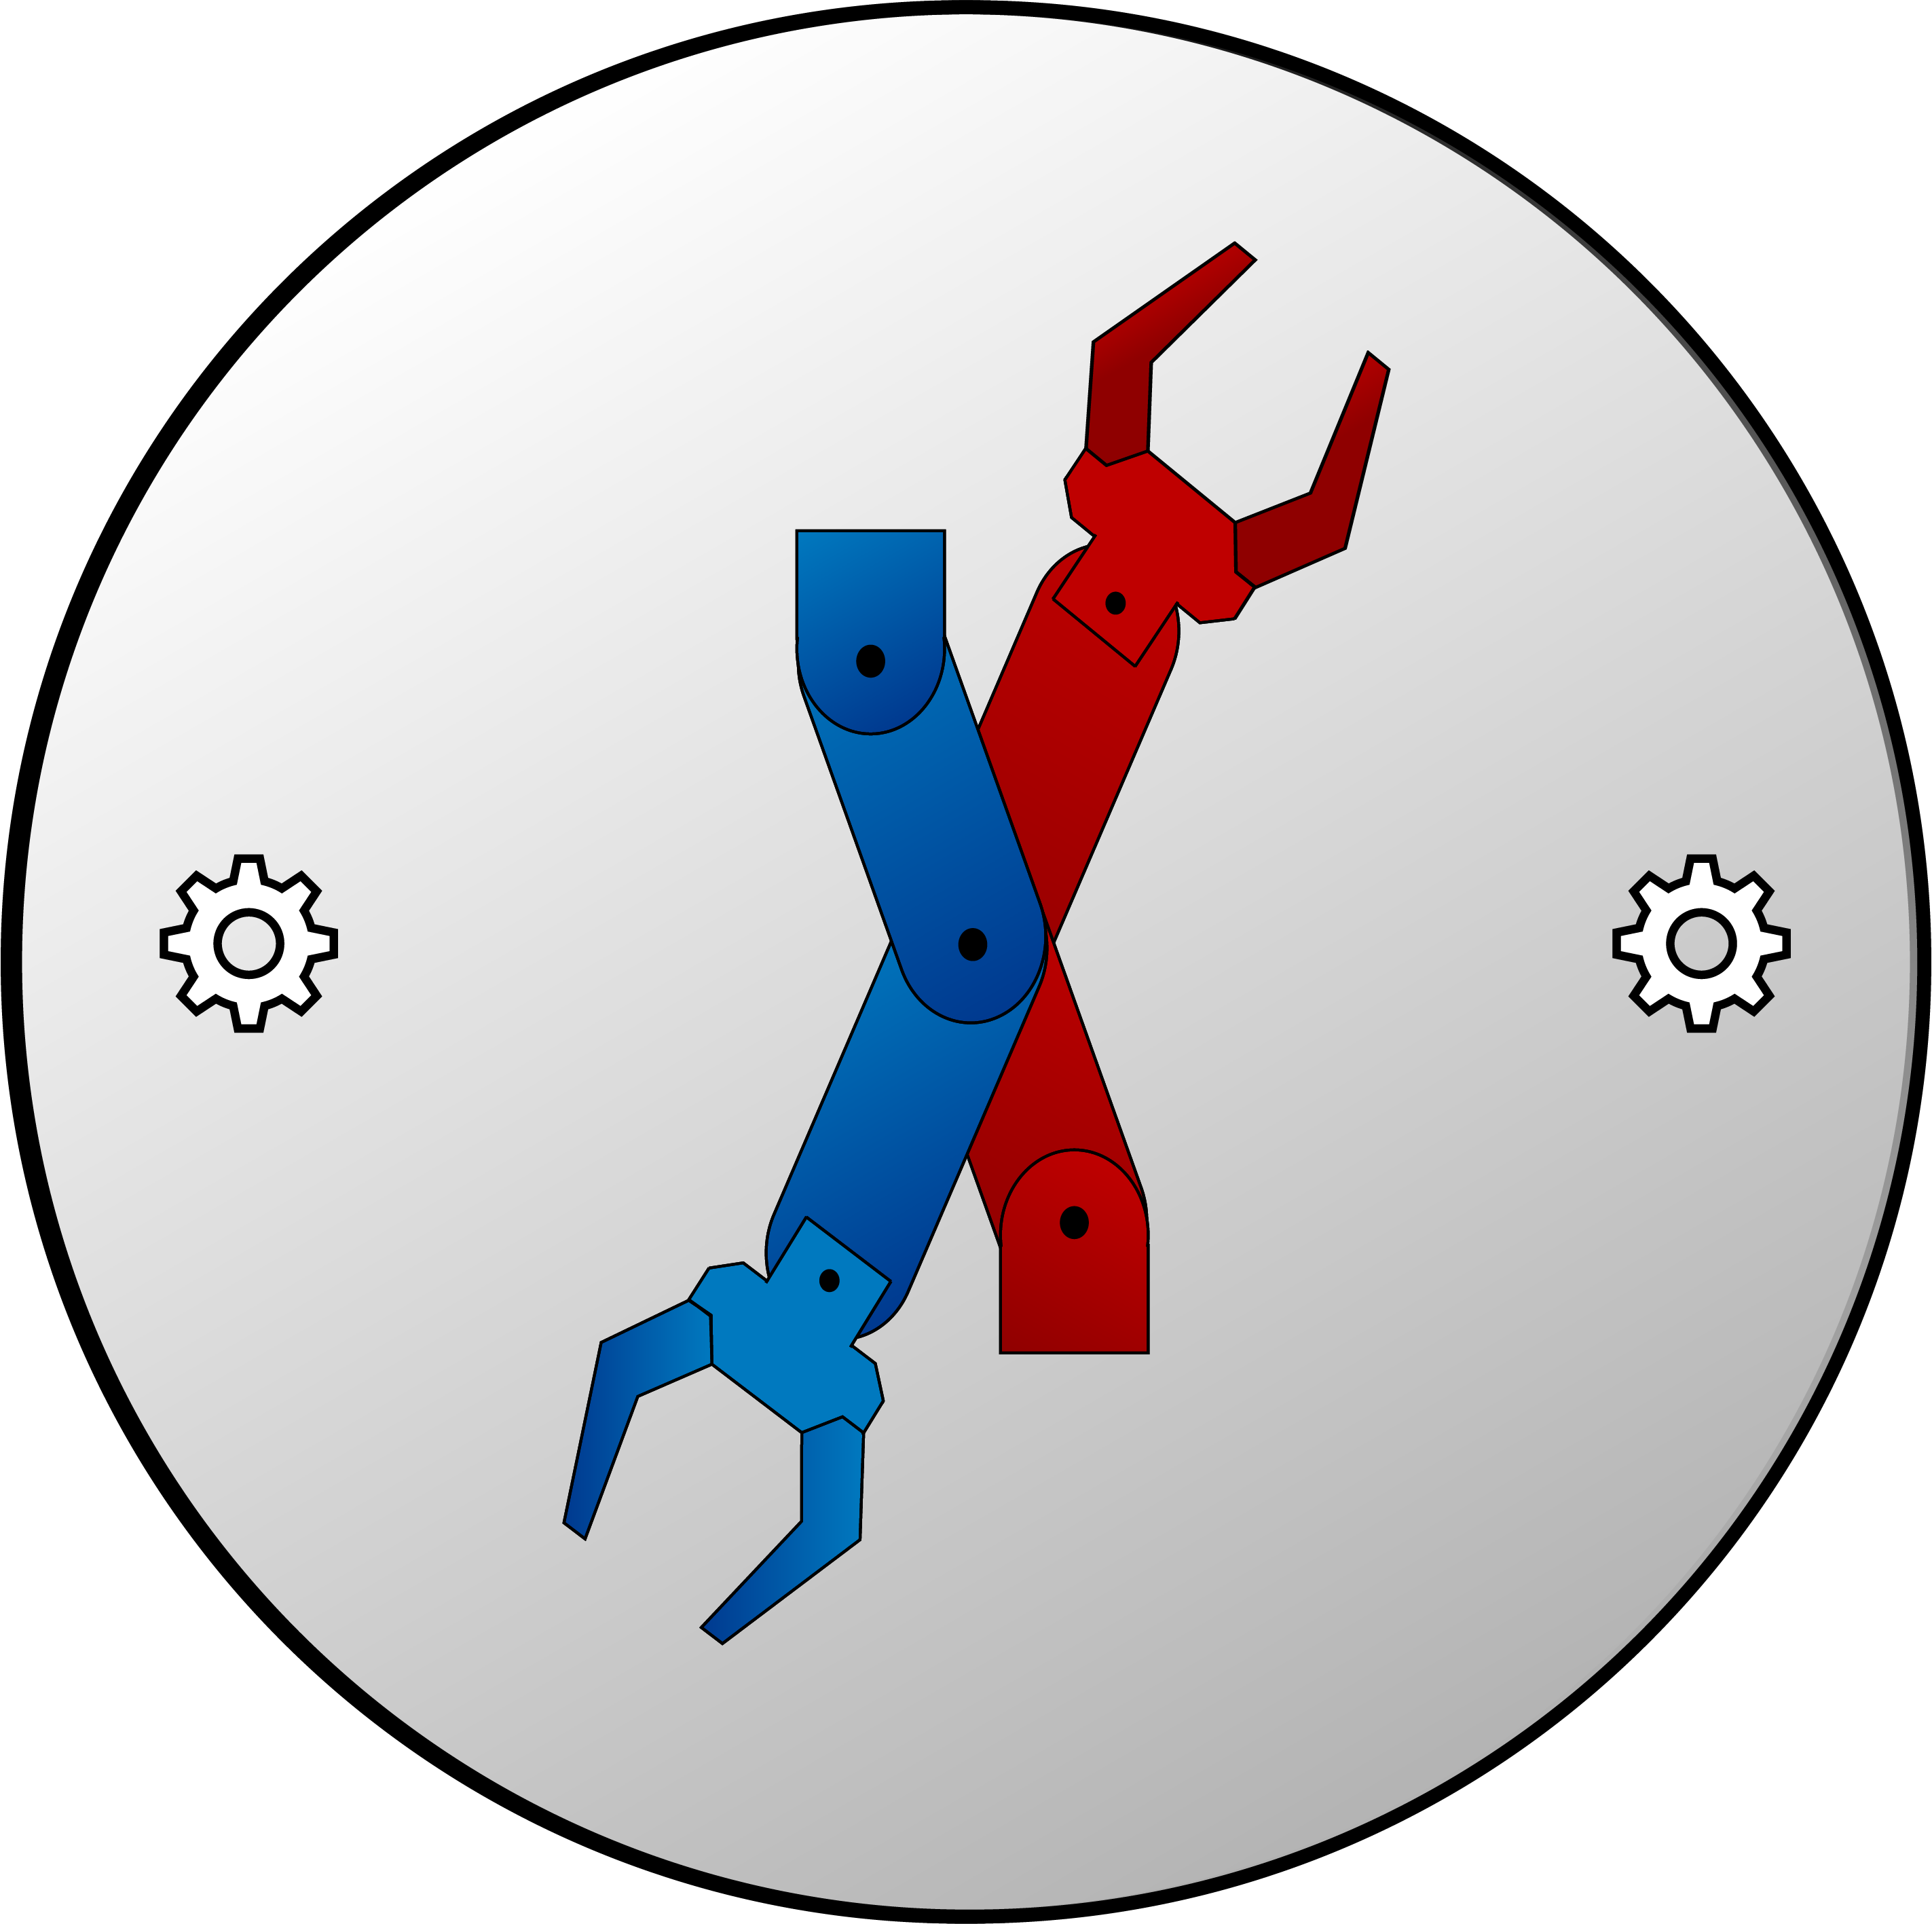
\includegraphics[width=.45\textwidth]{logo}
\vfill
\flushleft
ME 407 \\
Preliminary Design of Robotic Systems \\
Embry-Riddle Aeronautical University \\
\vspace{2ex}
\begin{minipage}[c]{.5\textwidth}
\flushleft

\includegraphics[width=.95\textwidth]{erau}
\end{minipage}%
\begin{minipage}[c]{.5\textwidth}
\flushright

\includegraphics[width=.8\textwidth]{text}
\end{minipage}
\end{titlepage}

\pagenumbering{roman}
\begin{abstract}
\color{red} ($\uparrow$ bold) 12pt times new roman centered horiz \& vert, full line space between header and text \color{black}
\blindtext
\vfill \begin{center} \color{red} no page number \color{black} \end{center}
\end{abstract}
{\tableofcontents\let\clearpage\relax\listoffigures\let\clearpage\relax\listoftables}
\vspace{2ex}

\color{red} latex table of contents, list of figures and table format with report document style\color{black}
\vfill
\begin{center}
\color{red} centered page numbers, roman numeral for frontmatter, arabic for rest\color{black}
\end{center}
\clearpage
\newpage

\section*{List Of Acronyms and Abbreviations}
\color{red} ($\uparrow$ bold) 12pt times new roman centered horiz \& vert, full line space between header and text \color{black}

\begin{tabular}{rl}
  $G$~:&Center of gravity of the bar \\
  $\ell_0$~:& Spring unstretched length  \\
  $\delta$~:& Spring deflection \\
  $k$~:& Spring constant \\
  $h_{b}$~:& Distance to bar ($G$) from datum \\
  $F_s$~:& Force onto bar due to spring\\
  $A_{n}$~:& Pin reaction in $\theta$ direction\\
  $A_{t}$~:& Pin reaction in tangential direction \\
  $\vec{v}_G$~:& Velocity of bar center of gravity\\
  $\ddot{\theta}$~:& Angular velocity of spring \\
  $\ddot{\phi}$~:& Angular velocity of bar\\
  $\ddot{\ell}_s$~:& Radial acceleration of spring \\
\end{tabular}

\vfill
\color{red}$\leftarrow$ \hfill margins 1 inch all around $\rightarrow$ \color{black}
\vfill\null

\normalsize
\flushleft
\singlespacing
\newpage
\pagenumbering{arabic}

\section{A Level Heading}

\color{red} $\uparrow$ left adjusted all headings arabic numbering ,full line space between headers and text \color{black}
\blindtext \cite{DBLP:journals/corr/JohnsonAL16} \color{red} 12pt. Times New Roman single spaced \color{black}
\section{A Level Heading}
\blindtext \cite{DBLP:journals/corr/RonnebergerFB15}
\subsection{B Level Heading}
\blindtext \cite{DBLP:journals/corr/abs-1803-09820}
\subsubsection{C Level Heading}
\blindtext
\subsubsection{C Level Heading}
\blindtext

\subsection{Example for Bulleted List}
\color{red} bullets are 3 dashed lines \color{black}
\blinditemize
\subsection{Example for Numbered List}
\blindenumerate
\subsection{Example for Descriptive List}
\blinddescription

\section{A Level Heading}
\blindtext

\begin{table}[htp]
  \center
  \caption{DH Table for 6 DOF Manipulator}
  \label{table:dh}
  \color{red} bold col headers, table times new roman, 12pt., centered, \color{black} \\
  \begin{tabular}{C{1cm}|C{1cm}C{2cm}C{1cm}C{1cm}}
    \textbf{DH} & $d_i$ & $\theta_i$ & $a_i$ & $\alpha_i$ \\ \hline
    1 & 280 & $q_1 - \pi$ & 0 & $\sfrac{\pi}{2}$ \\
    2 & 0 & $q_2 + \sfrac{\pi}{2}$ & 210 & 0 \\
    3 & 0 & $q_3 - \sfrac{\pi}{2}$ & 75 & -$\sfrac{\pi}{2}$ \\
    4 & 210 & $q_4$ & 0 & $\sfrac{\pi}{2}$ \\
    5 & 0 & $q_5 - \pi$ & 0 & $\sfrac{\pi}{2}$ \\
    6 & 70 & $q_6$ & 0 & 0 \\
  \end{tabular}
\end{table}

\emph{Table \ref{table:dh}} (\color{red} italisized callouts\color{black})shows the Denavit–Hartenberg parameters for the manipulator. \blindtext

Taking the time derivative,
$$
\vec{v}_G =
\left[\dot{\ell}_s\sin(\theta) + \frac{\ell_b\dot{\phi}\cos(\phi)}{2} +
\ell_s\dot{\theta}\cos(\theta)\right]\hat{\textrm{\i}} +
\left[\frac{\ell_b\dot{\phi}\sin(\phi)}{2} -
\dot{\ell}_s\cos(\theta) + \ell_s\dot{\theta}\sin(\theta)\right]\hat{\textrm{\j}}
$$
Since the moment of inertia $I$ for a uniform slender bar rotating about its end is
$\dfrac{1}{12}m\ell^2$ and $\omega = \dot{\phi}$,
$$T_2 = \frac{1}{2}m_{b}(\vec{v}_G \cdot \vec{v}_G) + \frac{1}{24}m_{b}\ell_b^2\dot{\phi}^2$$
Total Kinetic Energy: \hfill \color{red} equations 12pt, centered, numbered on right\color{black} \hfill\null
\begin{equation}
T = T_1 + T_2 = \frac{1}{2}m_{b}(\vec{v}_G \cdot \vec{v}_G) + \frac{1}{24}m_{b}\ell_b^2\dot{\phi}^2
\end{equation}

\begin{equation}
\ddot{\theta} = \frac{d}{dt}\left(\frac{\partial\Lag}{\partial\dot{\theta}}\right) -
\frac{\partial\Lag}{\partial\theta} = \big(Q_{\theta}\big)_{\text{non}}
\label{eq:lagtheta}
\end{equation}
\begin{equation}
\ddot{\phi} = \frac{d}{dt}\left(\frac{\partial\Lag}{\partial\dot{\phi}}\right) -
\frac{\partial\Lag}{\partial\phi} = \big(Q_{\phi}\big)_{\text{non}}
\label{eq:lagphi}
\end{equation}

\section{A Level Heading}
\blindtext
\newpage
\begin{figure}[h]
  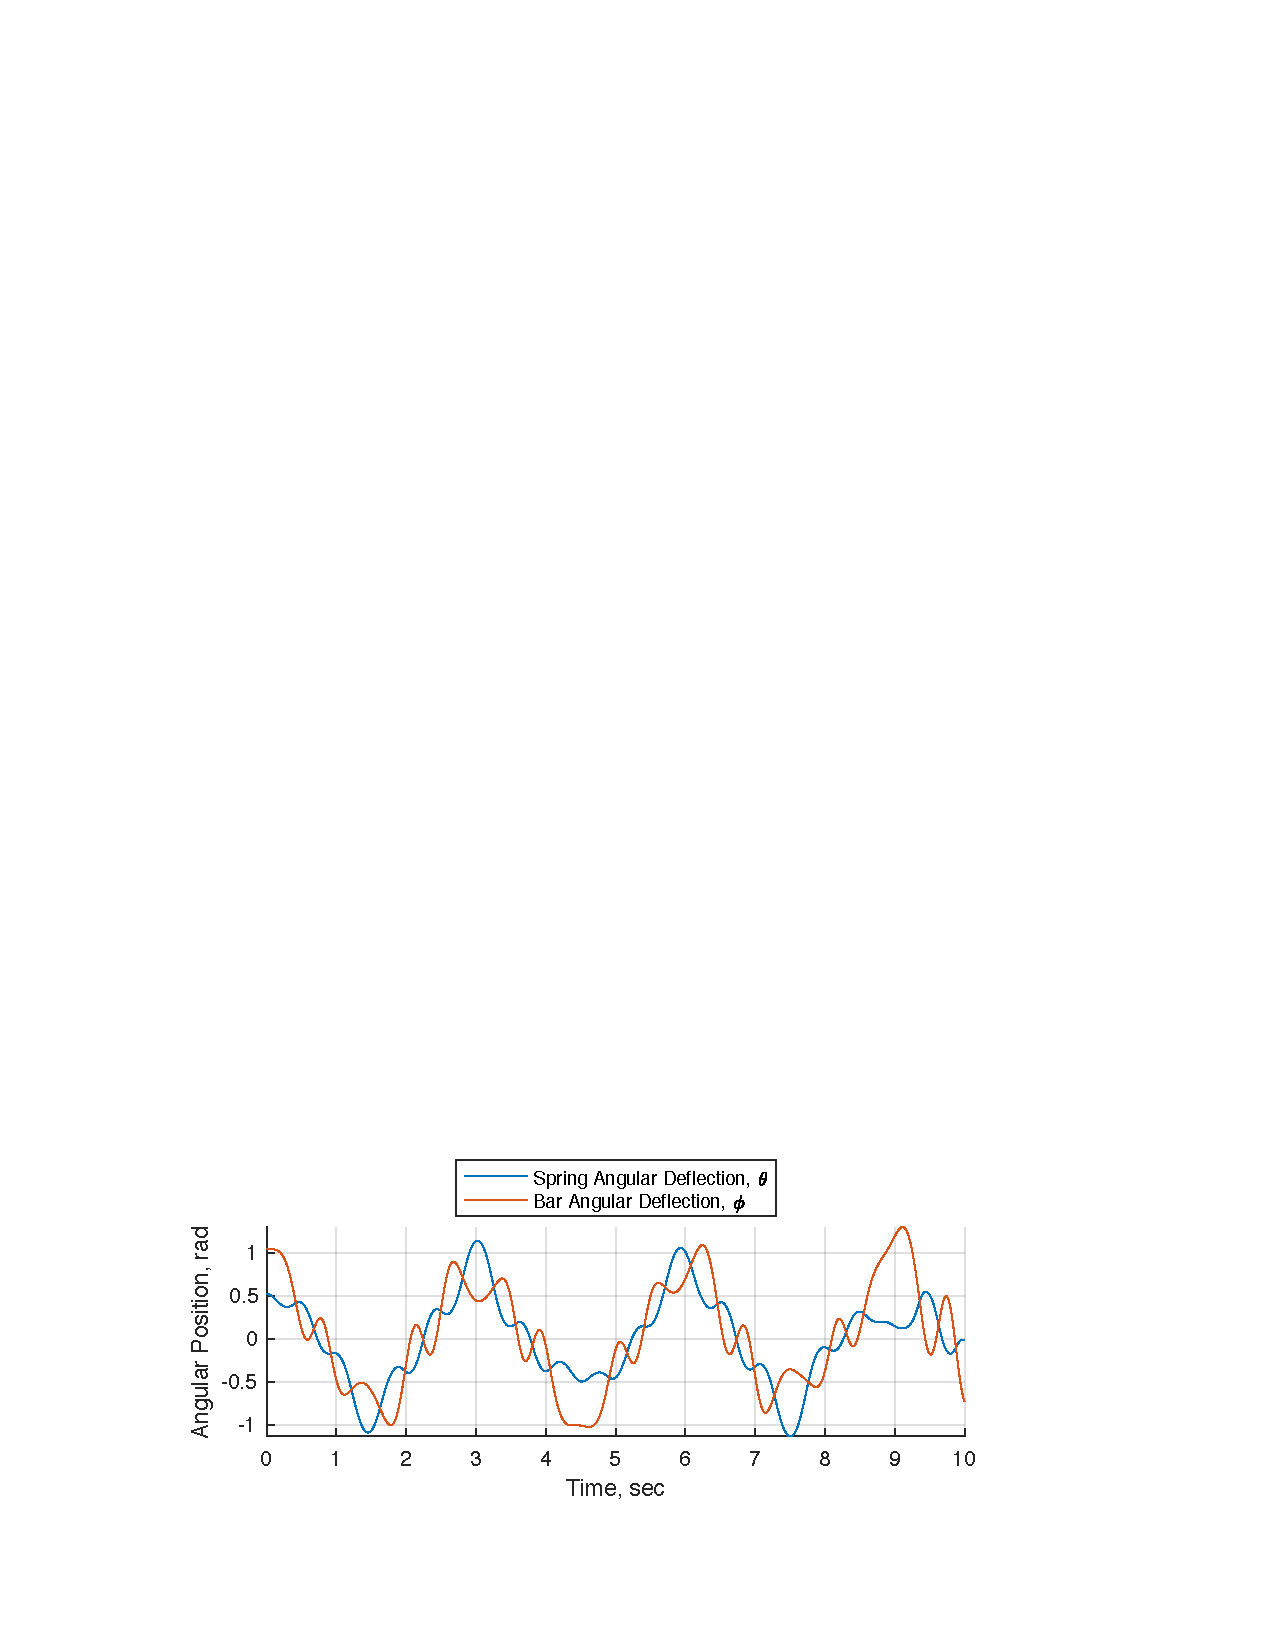
\includegraphics[center]{spring_0-0}
  \caption{Numerical Solution Motion Behavior Plot, ($\theta_o:~0,~\phi_o:~0$)}
  \label{fig:spring}
\end{figure}

\emph{Figure \ref{fig:spring}} shows the relationship between \blindtext
\newpage
\section{A Level Heading}
\begin{figure}[h]
  \centering
  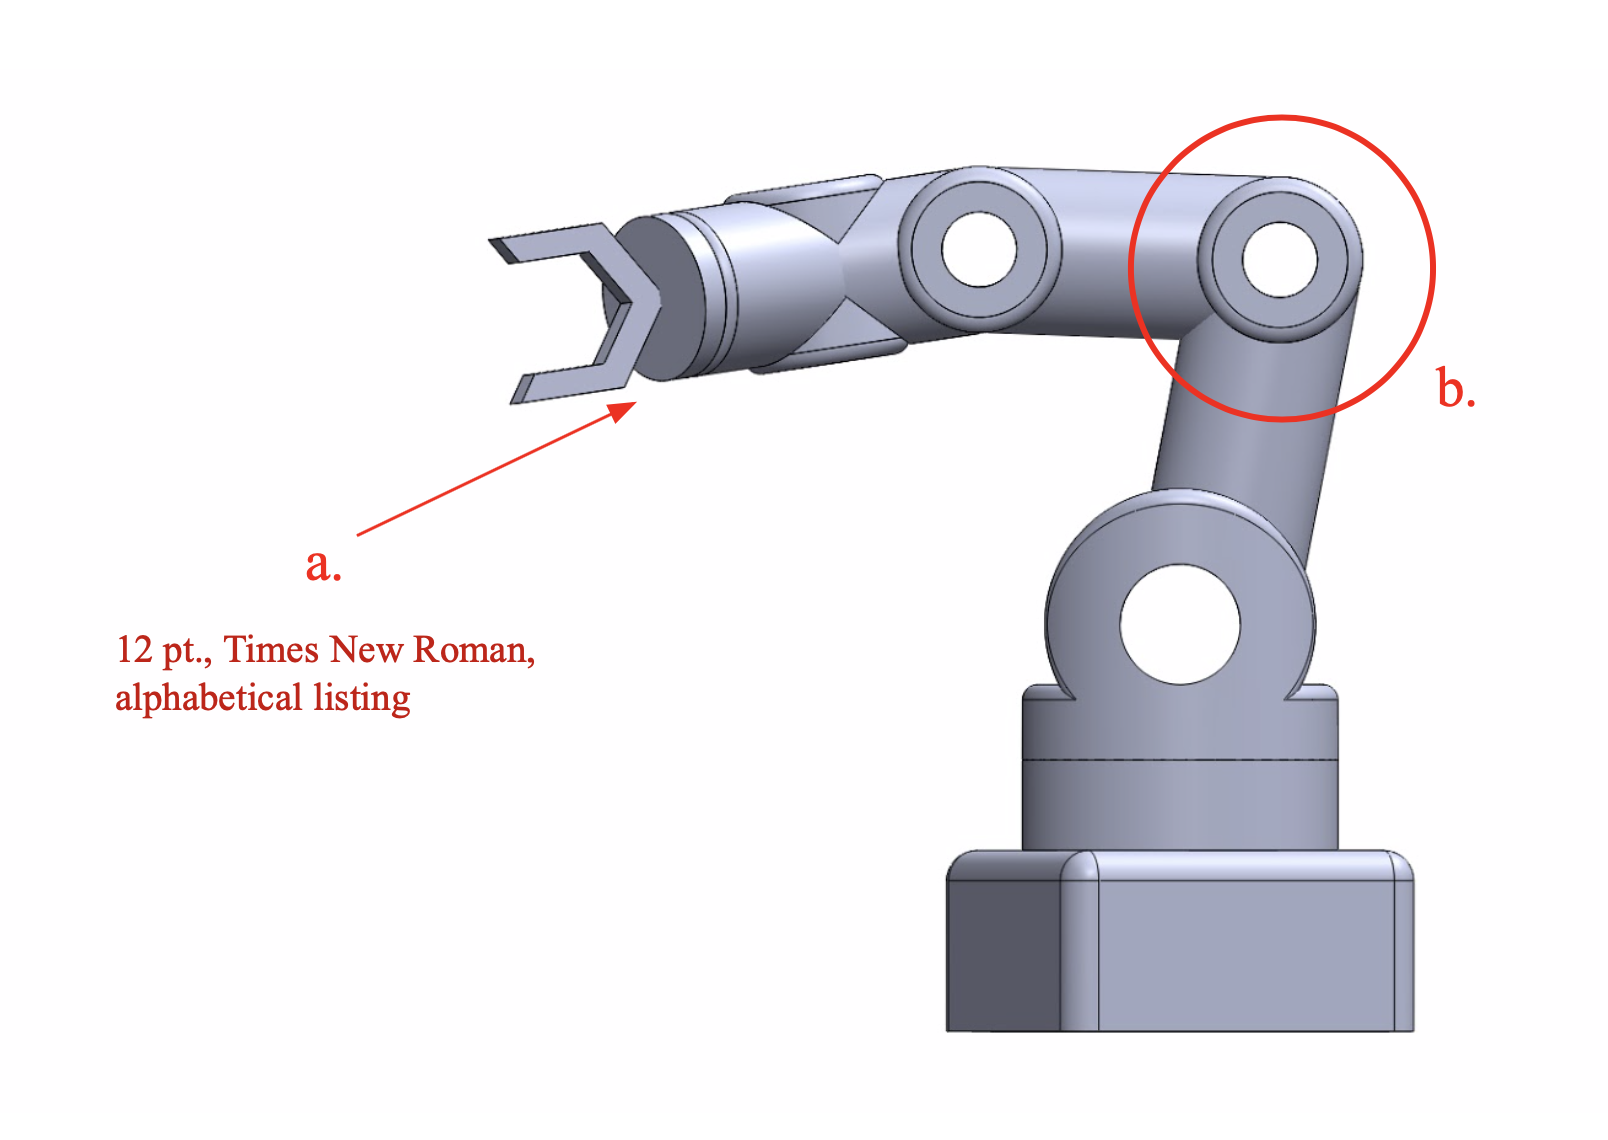
\includegraphics[width=.75\textwidth]{callouts}
  \caption{Figure with Callouts}
  \label{fig:callouts}
\end{figure}

\begin{enumerate}[label=\alph*.]
  \item Description for callout a
  \item Description for callout b
\end{enumerate}

As seen in \emph{Figure \ref{fig:callouts}}, callout a. is blah. \\
\blindtext

\newpage
\bibliographystyle{plain}
\bibliography{JohnsonAL16,abs-1803-09820,RonnebergerFB15}
\vspace{2ex}

\color{red}
12pt times new roman left justified \\
all references follow IEEE formatting
\color{black}

\newpage
\section*{Acknowledgements \& Attributions}
\blinditemize
\newpage

\newpage
\appendix
\renewcommand\thesection{\Roman{section}}
\renewcommand\thesubsection{\roman{subsection}}
\section*{Appendix}\label{sec:app}
\begin{lstlisting}[frame=lines,style=Matlab-editor,basicstyle = \mlttfamily, caption=Example Code Listing]
Lagrangian = T - V;
% Partial of Lagrange Eq. w.r.t. thetadot
dLdthetadot = diff(Lagrangian,thetadot);
dLdthetadot_subbed = subs(dLdthetadot, [thetat, thetadot, phit, phidot,...
   l1t, l1dot], [theta, diff(theta,t), phi, diff(phi,t), l1, diff(l1,t)]);
% Time derivative of Partial of Lagrange Eq. w.r.t. thetadot
ddLdthetadotdt = diff(dLdthetadot_subbed,t);
% Partial of Lagrange Eq. w.r.t. theta
dLdtheta = diff(Lagrangian,thetat);
% Theta EOM
eqn(1) = ddLdthetadotdt - dLdtheta == 0;
\end{lstlisting}

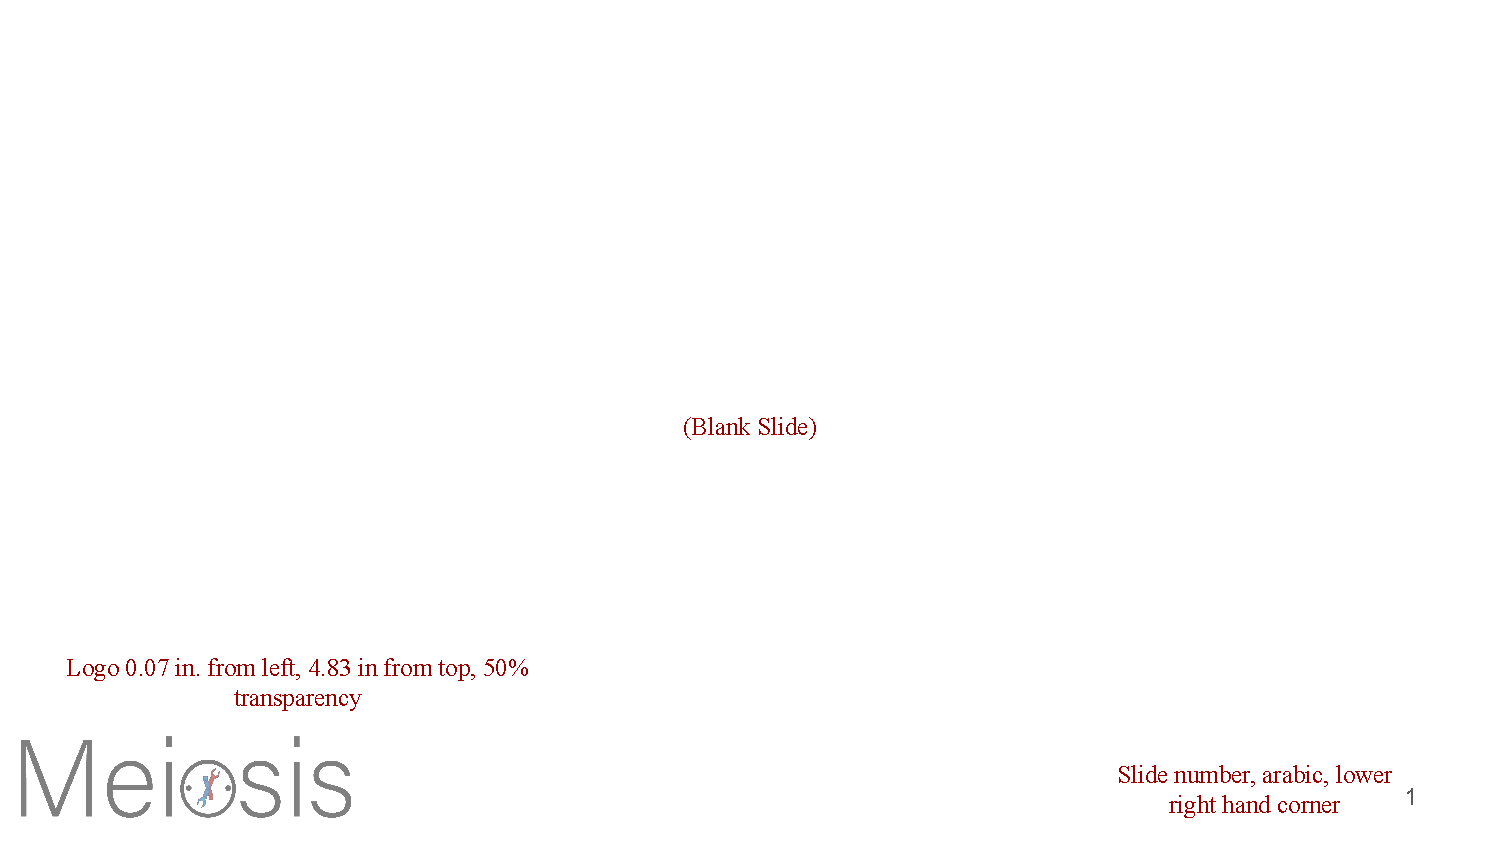
\includepdf[landscape,pages=-]{presentation}

\end{document}
